\documentclass{article}
\usepackage{graphicx}
\usepackage{float}

\begin{document}

\title{Current Thesis Progress}
\author{Abdul Tawab Ajmal Safi}

\maketitle

% \begin{abstract}
% What the hell is going on!!!!!
% \end{abstract}

\section{Currency Portfolios for Carry Trade}
According to the Uncovered Interest Rate Parity (UIP) the interest rate differential between two countries
will be equal to the relative change in currency exchange rates over the same period. This theory does not hold in reality
as exchange rates appear to move in the opposite direction of the interest rate differential between two countries. Creating an
arbitrage opportunity to make profit by borrowing from countries with low interest rate and lending to countries with high
interest rate to earn a profit based on the interest rate differential. In this paper, I am going to consider multiple portfolio creation
and optimization strategies that can be used for carry trade.


\subsection{Variables of Interest}
\begin{itemize}
  \item Short and Long Term Country Yields
  \item Short and Long Term Expectation Component for Yields
  \item Short and Long Term Risk Premium Component for Yields
  \item FOREX news articles
  \item Exchange Rates (Base currency is USD)
  \item Countries being considered: [AUS ,  CAN ,  CHI ,  CHN ,  COL ,  CZR ,  EUR ,  HUN ,
                       INDO ,  JAP ,  MEX ,  NOR ,  NZ ,  PO , SA ,  SNG , SWE ,  SWI ,  UK  , BRA]
  \item Date Range: Monthly Data from 2007 to 2019
\end{itemize}

\newpage

\subsection{Portfolio Creation Based on Interest Rate Differential}
In this section, I used python code to create a carry trade simulation by organizing countries into portfolio's
based on their interest rate differential with USA and then using historic data to trade on varying time intervals
to see how profit from carry trade changes based on the weights and trade intervals being used for portfolio generation.
It is important to note that the calculation of profit in carry trade does not take into account the transaction cost.

\subsubsection{Basic Procedure}

\begin{itemize}
  \item Initialize individual trade interval (i.e daily, monthly, quarterly or annual trading)
  \item Sort foreign currencies into portfolios based on their interest rate differential with USA.
  \item Assign weights to currencies for portfolio optimization.
\end{itemize}

\subsubsection{Return on Trading for Monthly Basis}

\vspace*{-6.8mm}

\begin{figure}[H]
    \centering
    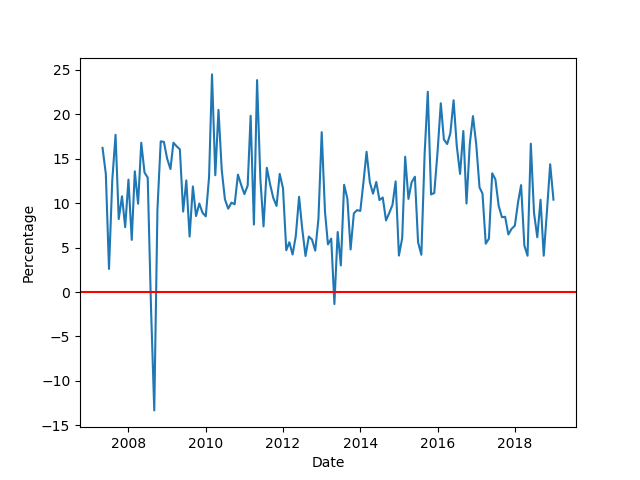
\includegraphics[scale=.75]{images/carryTrade/monthly1.png}
    \caption{Percentage Profit From Monthly Carry Trade (Weight = [100])}
    \label{simulationfigure}
\end{figure}

\begin{itemize}
  \item Average Percentage profit: 10.89
  \item The strategy makes the biggest loss around 2008, which was during the financial crisis.
  \item The biggest loss of the strategy is about 10 percentage point smaller than the biggest profit.
  \item In order to get rid of loss it might be a good idea to diversify our portfolio by assigning weights.
\end{itemize}

\begin{figure}[H]
    \centering
    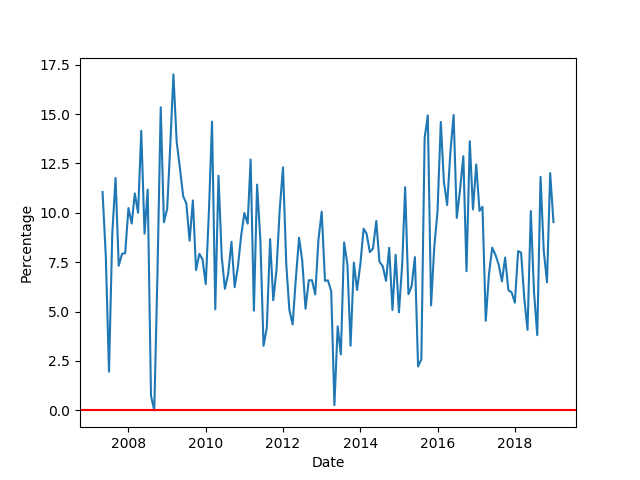
\includegraphics[scale=.75]{images/carryTrade/monthly2.png}
    \caption{Percentage Profit From Monthly Carry Trade (Weight = [40,30,30])}
    \label{simulationfigure}
\end{figure}

\begin{itemize}
  \item Average Percentage profit: 8.29
  \item Although our average profit reduced, our strategy does not face any major losses.
  \item Borrowing from multiple countries and lending to multiple countries has allowed us to reduce any potential risk and losses.
  \item A further step to this will be to come up with a dynamic system that automatically adjusts weights for short and long after every single trade.
  \item Another advancement that can be introduced is the use of dynamic trading intervals by allowing the algorithm to decide the best for going short and long.
\end{itemize}

\subsubsection{Return on Trading for Half Year(6 months) Basis}

\vspace*{-6.8mm}

\begin{figure}[H]
    \centering
    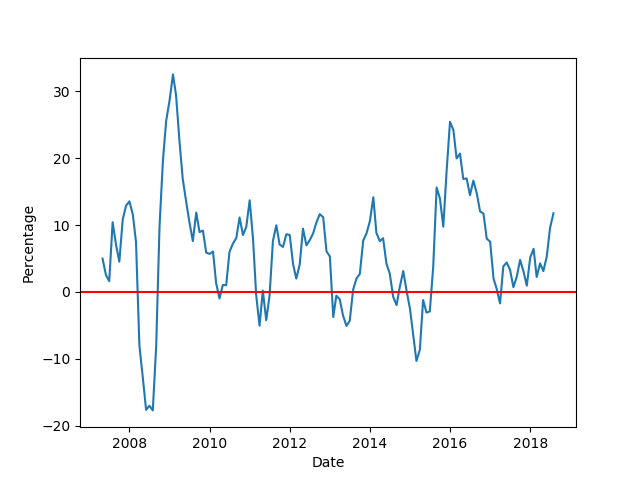
\includegraphics[scale=.75]{images/carryTrade/halfYear1.png}
    \caption{Percentage Profit From Half Year Carry Trade (Weight = [40,30,30])}
    \label{simulationfigure}
\end{figure}

\begin{itemize}
  \item Average Percentage profit: 6.17. (Lower than the monthly Average Percentage Return)
  \item The number of losses faced by the trading strategy increases as the trading interval increases from 1 month to 6 months.
  \item It appears to be more profitable and risk aversive to indulge in carry trade over monthly basis rather than half-year basis.
  \item This indicates that interest rate differential for carry trade is a more beneficial over shorter periods of time.
  \item UIP might come to hold over the long run making carry trade not profitable.
  \item Longer trade interval results in higher risk because half year is enough time for a country's economic situation to change.
  \item It will be interesting to see if introduction of dynamic weight portfolio optimization strategy will make carry trade also profitable over the long run.
\end{itemize}

% \begin{equation}
%     \label{simple_equation}
%     \alpha = \sqrt{ \beta }
% \end{equation}

\section{Predicting the Directional Change in Foreign Exchange Returns}

\subsection{Feature Engineering}

\vspace*{1mm}

\subsubsection{Monthly Exchange Rate Return}

\vspace*{2mm}

The equation below shows the exchange rate return that you gain if you go short on a currency one month after you bought it. This equation has been acquired from the following source:
https://www.investopedia.com/articles/forex/12/calculating-profits-and-losses-of-forex-trades.asp

\[return_t^i=\frac{er_t^i - er_{t+1}^i}{er_{t+1}^i}\]}

\begin{itemize}
  \item $\[er_t\]$ = is current exchange rate of a foreign currency (USD as base currency.)
  \item $\[er_{t+1}\]$ = one month ahead exchange rate of a foreign currency (USD as base currency.)
  \item superscript i indicates the country being considered
\end{itemize}


\begin{figure}[H]
    \centering
    \hspace*{-2.5in}
    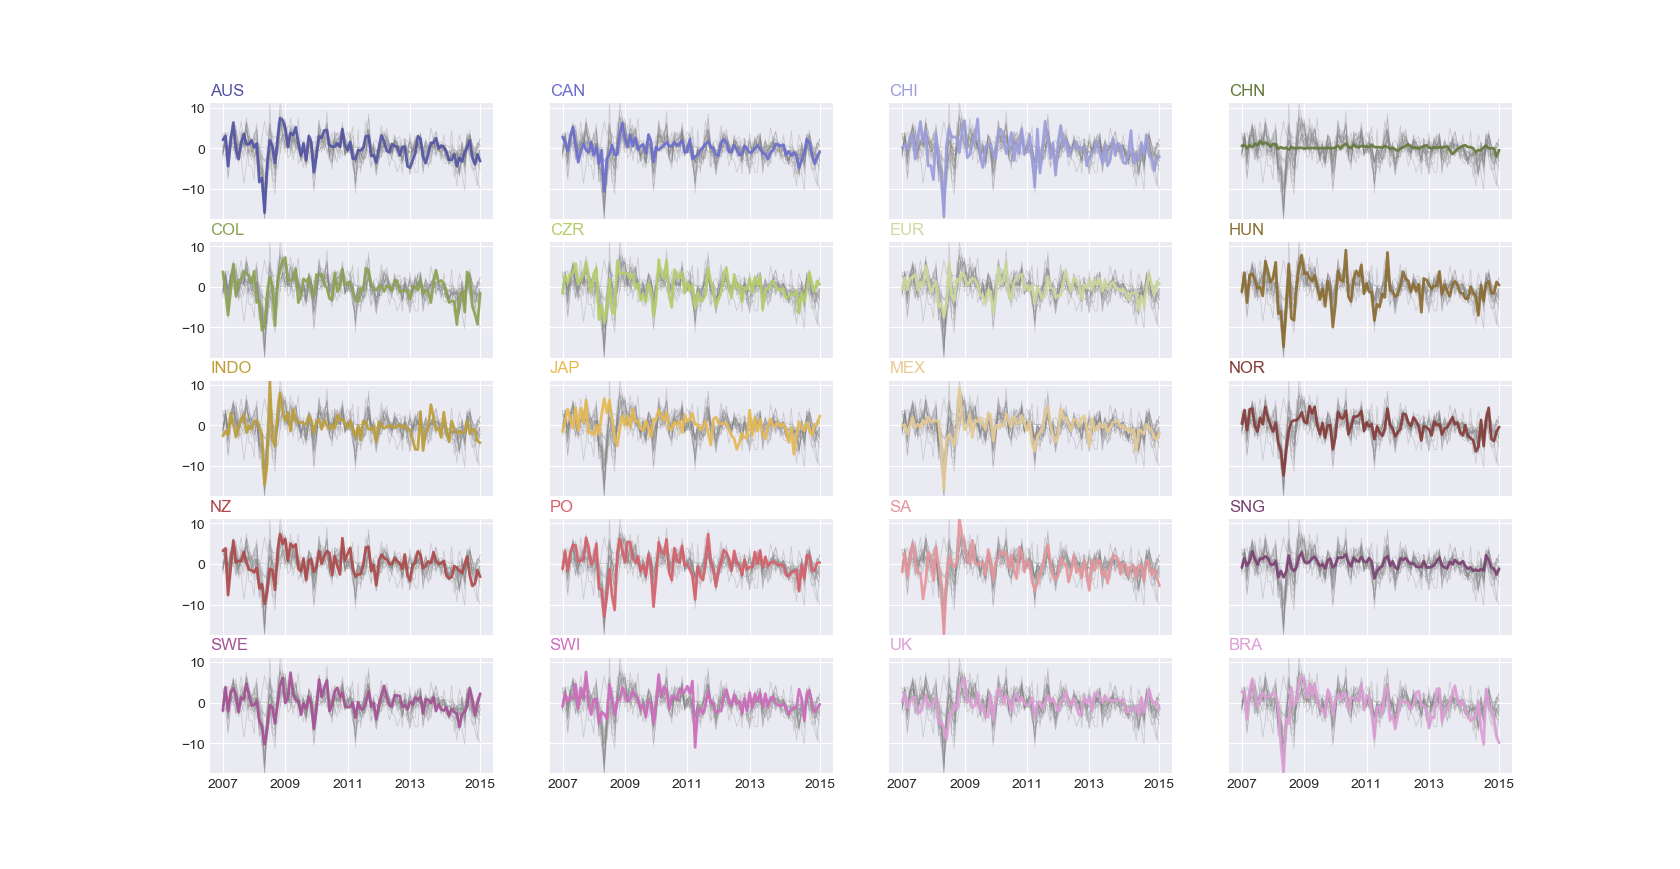
\includegraphics[scale = .58]{images/direction/er_return.png}
    \caption{Monthly Exchange Rate Return for all countries from 2007 to 2015}
    \label{simulationfigure}
\end{figure}

\begin{itemize}
  \item China appears to have the least volatility in exchange rate returns as their currency is pegged against USD.
  \item It is interesting to see how almost all currencies faced an instant fall in exchange rate returns during the 2008 financial crisis.
  \item Singapore appears to have the second least volatility in exchange rate returns after China.
\end{itemize}

\newpage

\subsubsection{Principal Component Analysis of Yield, Expectation and Term Premium}

\vspace*{5mm}

Our interest rate or yield data ranges from 2 months up until 120 months for each country. Similarly the term premium
and expectation component of yield curve also range from 2 months to 120 months for each country. In order to account for
all short and long term yield and its component's data, I take the first three principal components of all three variables for all countries.
On average the first three PCA describes more than 95 percent variance of all the variables. According to theory the first three principal components
of yield, expectation, and term premium account for the level, slope and curative of the variables respectively. The following nine variables were generated
after PCA:

\vspace*{5mm}
\begin{itemize}
  \item yield level
  \item yield slope
  \item yield curvature
  \item expectation level
  \item expectation slope
  \item expectation curvature
  \item term premium level
  \item term premium slope
  \item term premium curvature
\end{itemize}


\begin{figure}[H]
    \centering
    \hspace*{-2.5in}
    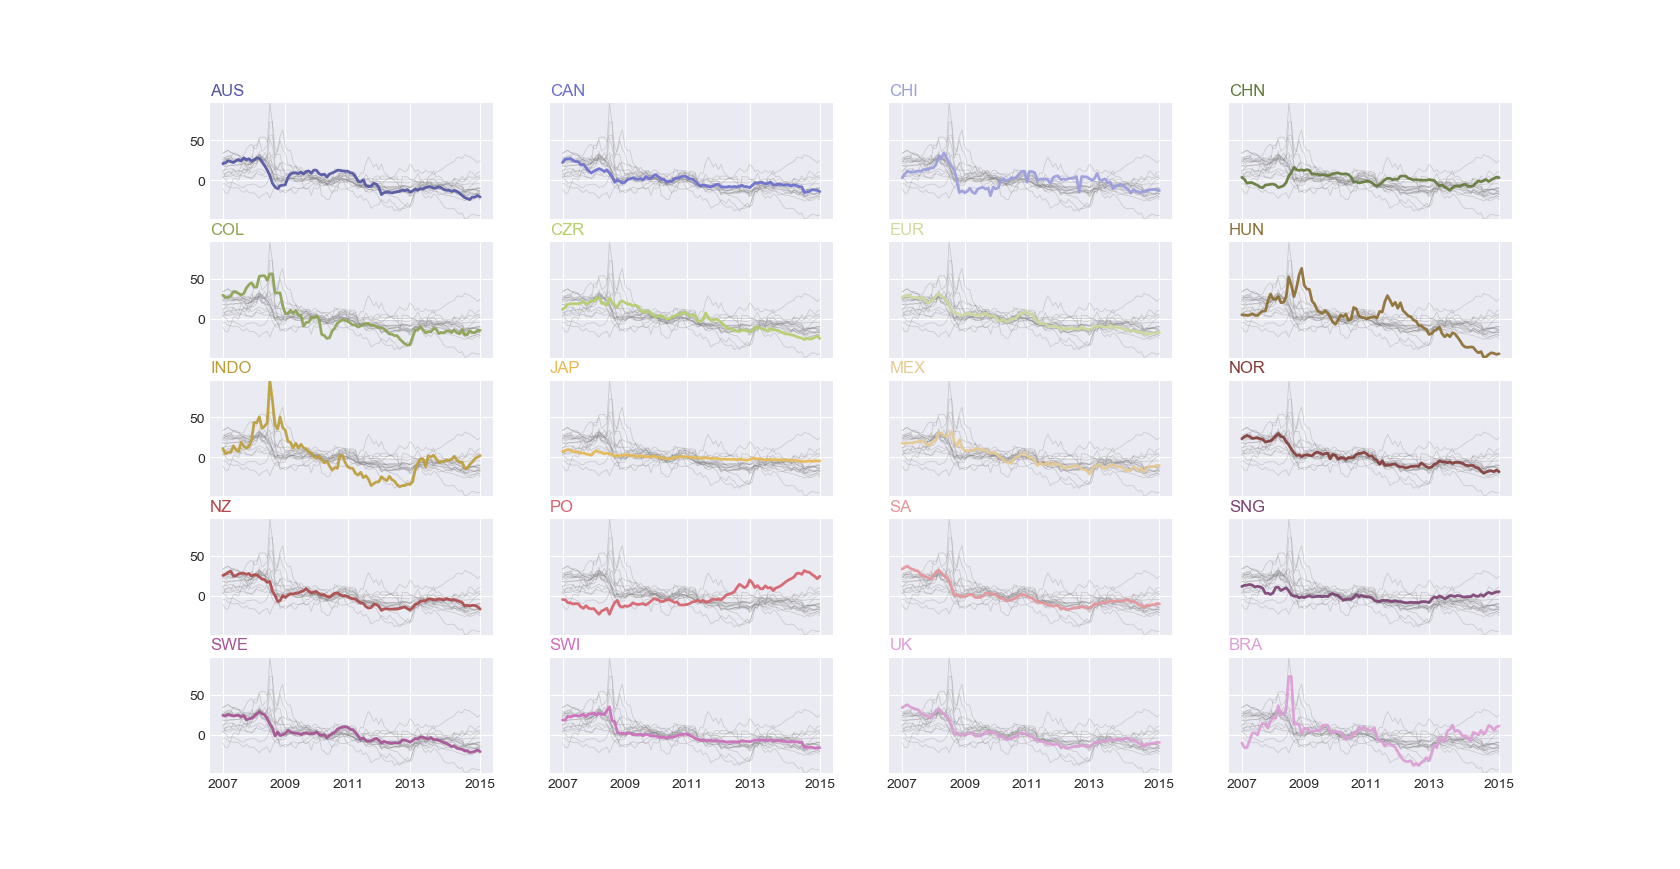
\includegraphics[scale = .58]{images/direction/yield_level.png}
    \caption{Yield Level for all countries from 2007 to 2015}
    \label{simulationfigure}
\end{figure}

\begin{figure}[H]
    \centering
    \hspace*{-2.5in}
    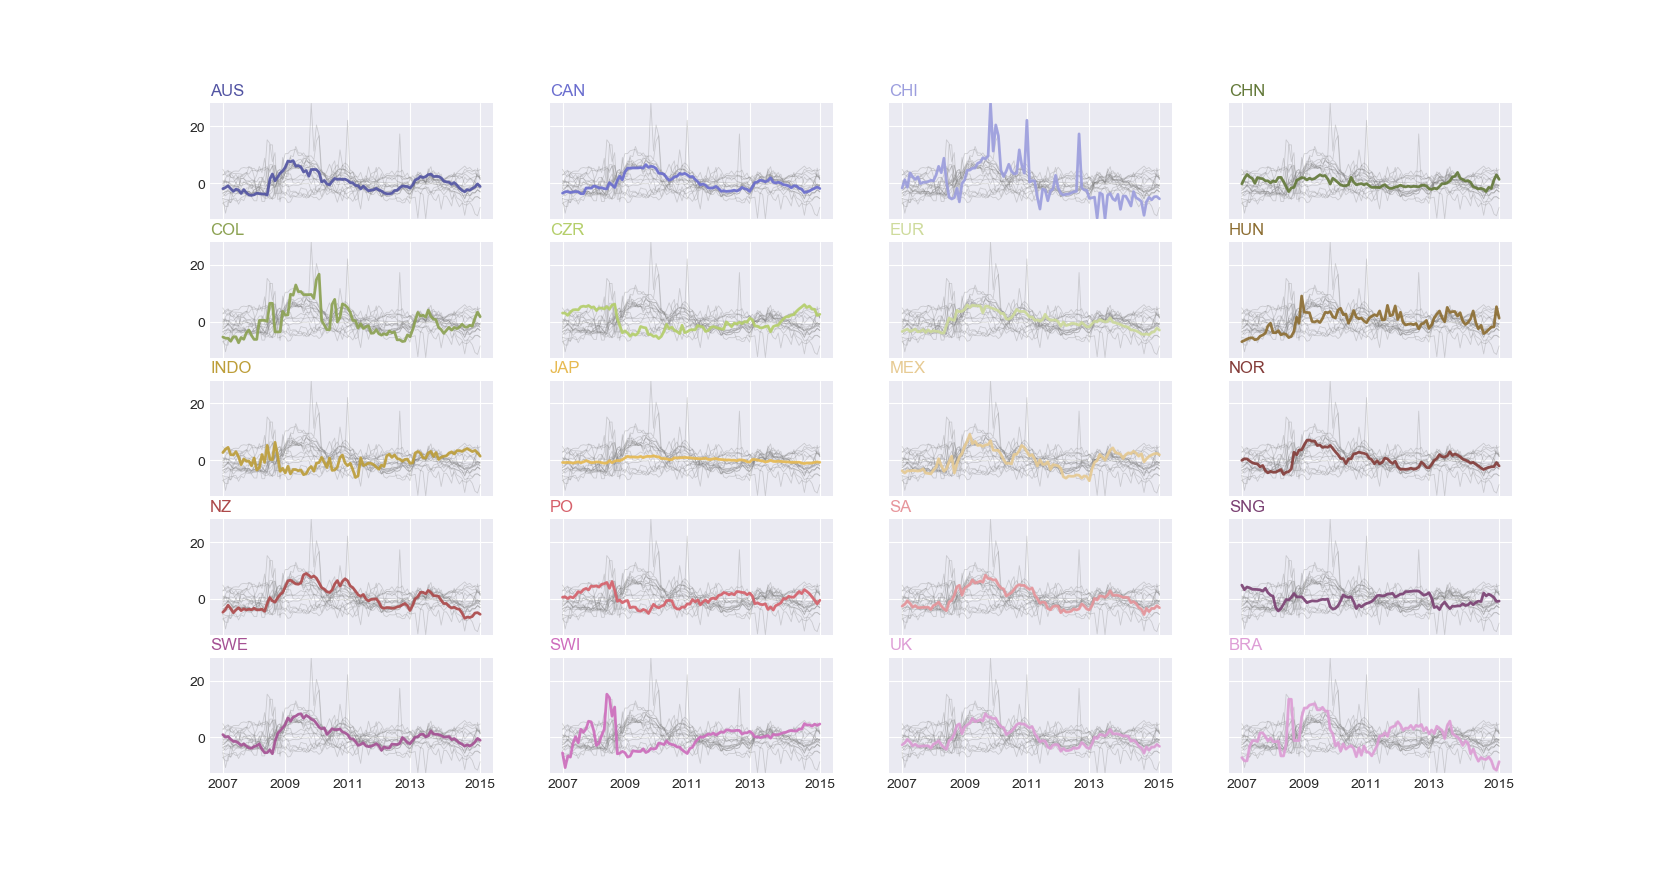
\includegraphics[scale = .58]{images/direction/yield_slope.png}
    \caption{Yield Slope for all countries from 2007 to 2015}
    \label{simulationfigure}
\end{figure}

\begin{figure}[H]
    \centering
    \hspace*{-2.5in}
    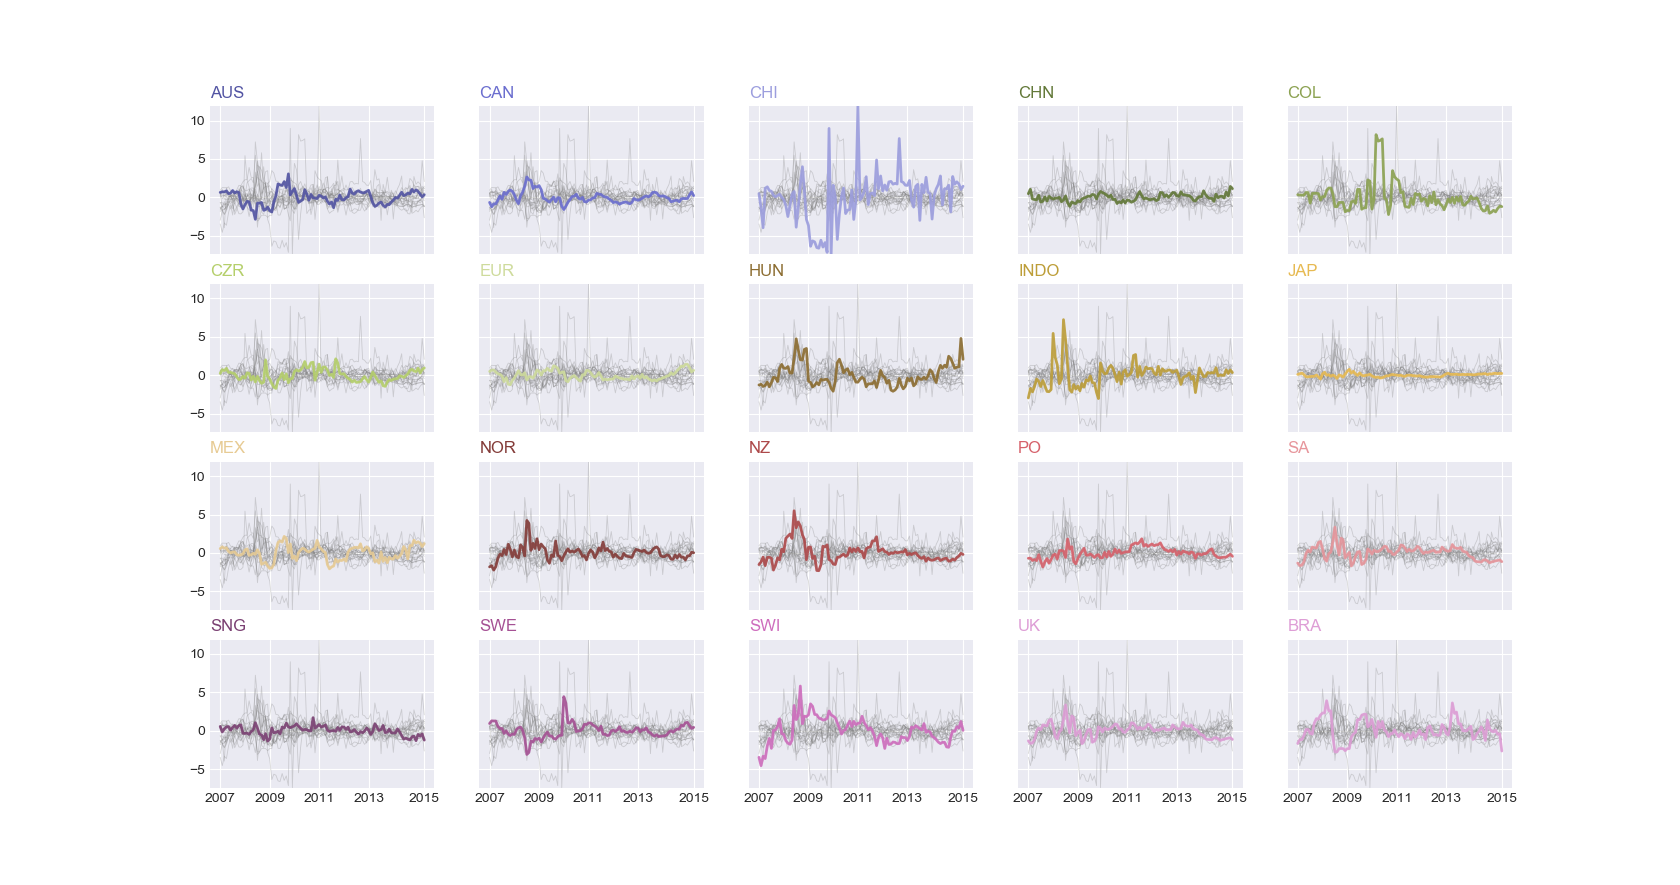
\includegraphics[scale = .58]{images/direction/yield_curvature.png}
    \caption{Yield Curvature for all countries from 2007 to 2015}
    \label{simulationfigure}
\end{figure}

\begin{itemize}
  \item China appears to be the most stable across all three components of yield.
  \item It is interesting to see how Chile appears relatively normal in yield level but faces drastically increased volatility in the slope and curvature component.
  \item Similar graphs for the expectation and term premium components were also created which can be included in the appendix.
\end{itemize}

\newpage

\subsection{Support Vector Machine for Buy/Sell Classification}
\vspace*{5mm}

\subsubsection{Setup}

\vspace*{5mm}

\begin{itemize}
  \item A 70/30 percent train/test split was created to check in and out of sample performance of our model.
  \item A binary column named "buy" was created which was given a value of 1 for one month ahead positive return and a 0 for one month ahead negative or zero return.
  \item A machine learning technique called Grid Search was used to find the best parameters for our support vector classifier. Grid Search fits model with different
  parameters and uses cross validation to find the best combination.
  \item Support Vector Classification Models were for all countries, and confusion matrix on the train and test datasets were used to check the performance of our models.
\end{itemize}

\begin{figure}[H]
    \centering
    \hspace*{-1.25in}
    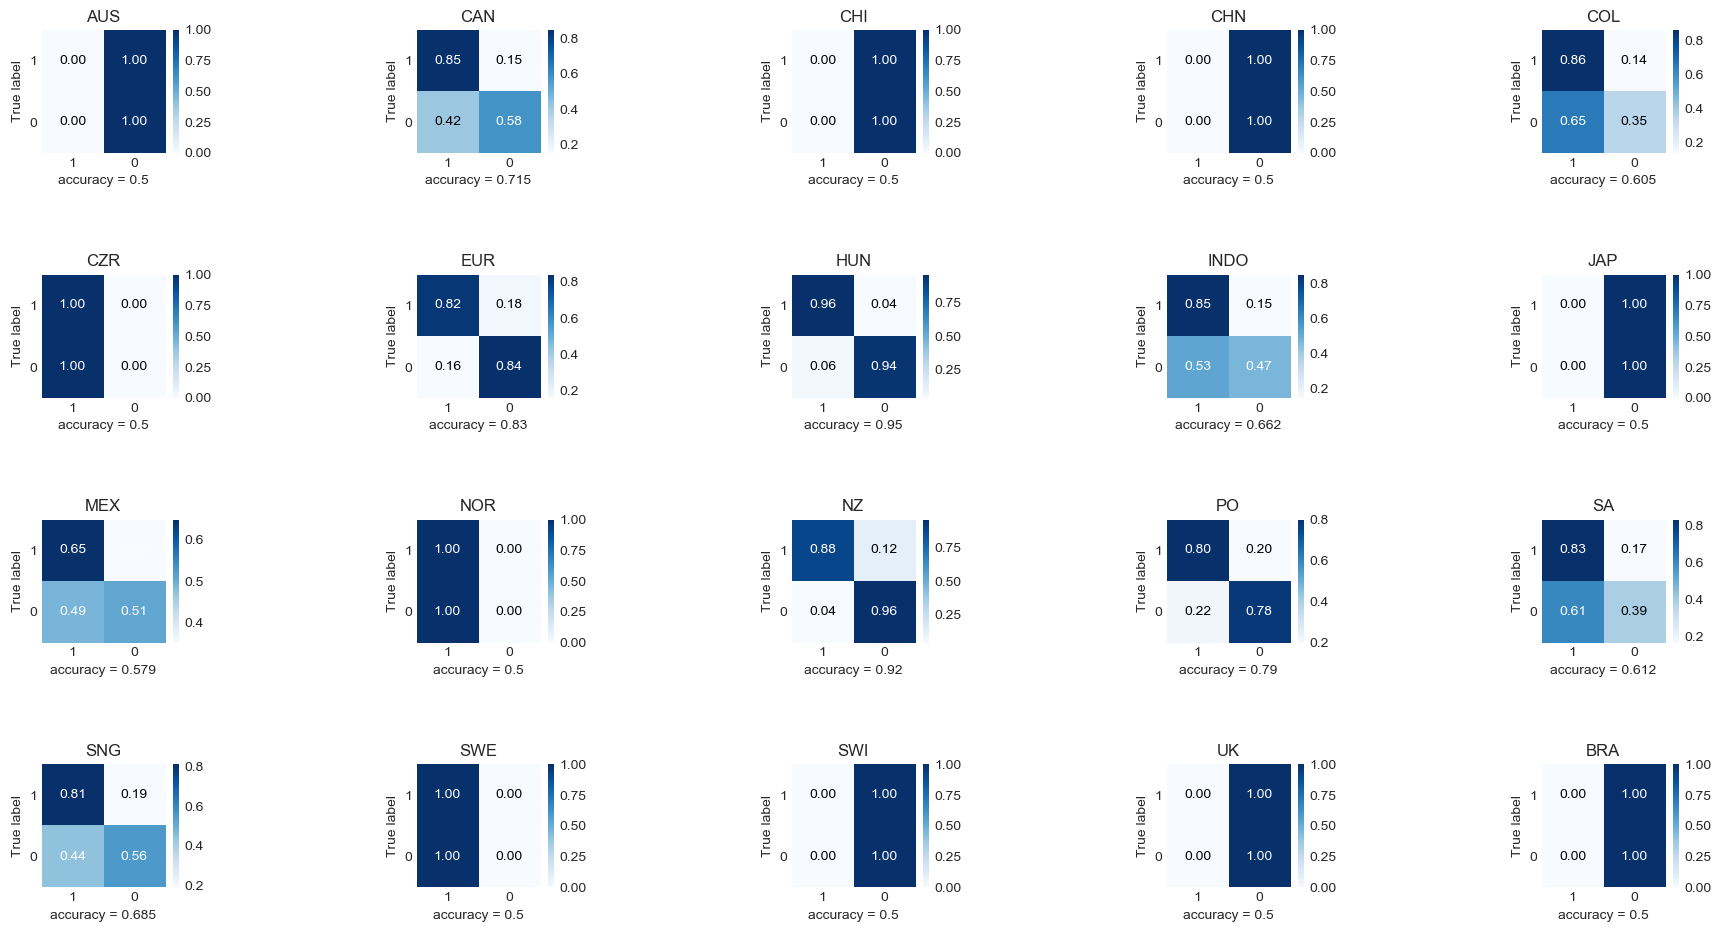
\includegraphics[scale = .30]{images/direction/clf_cm_train.png}
    \caption{SVC Confusion Matrix for all countries for Training Dataset}
    \label{simulationfigure}
\end{figure}

\begin{figure}[H]
    \centering
    \hspace*{-1.25in}
    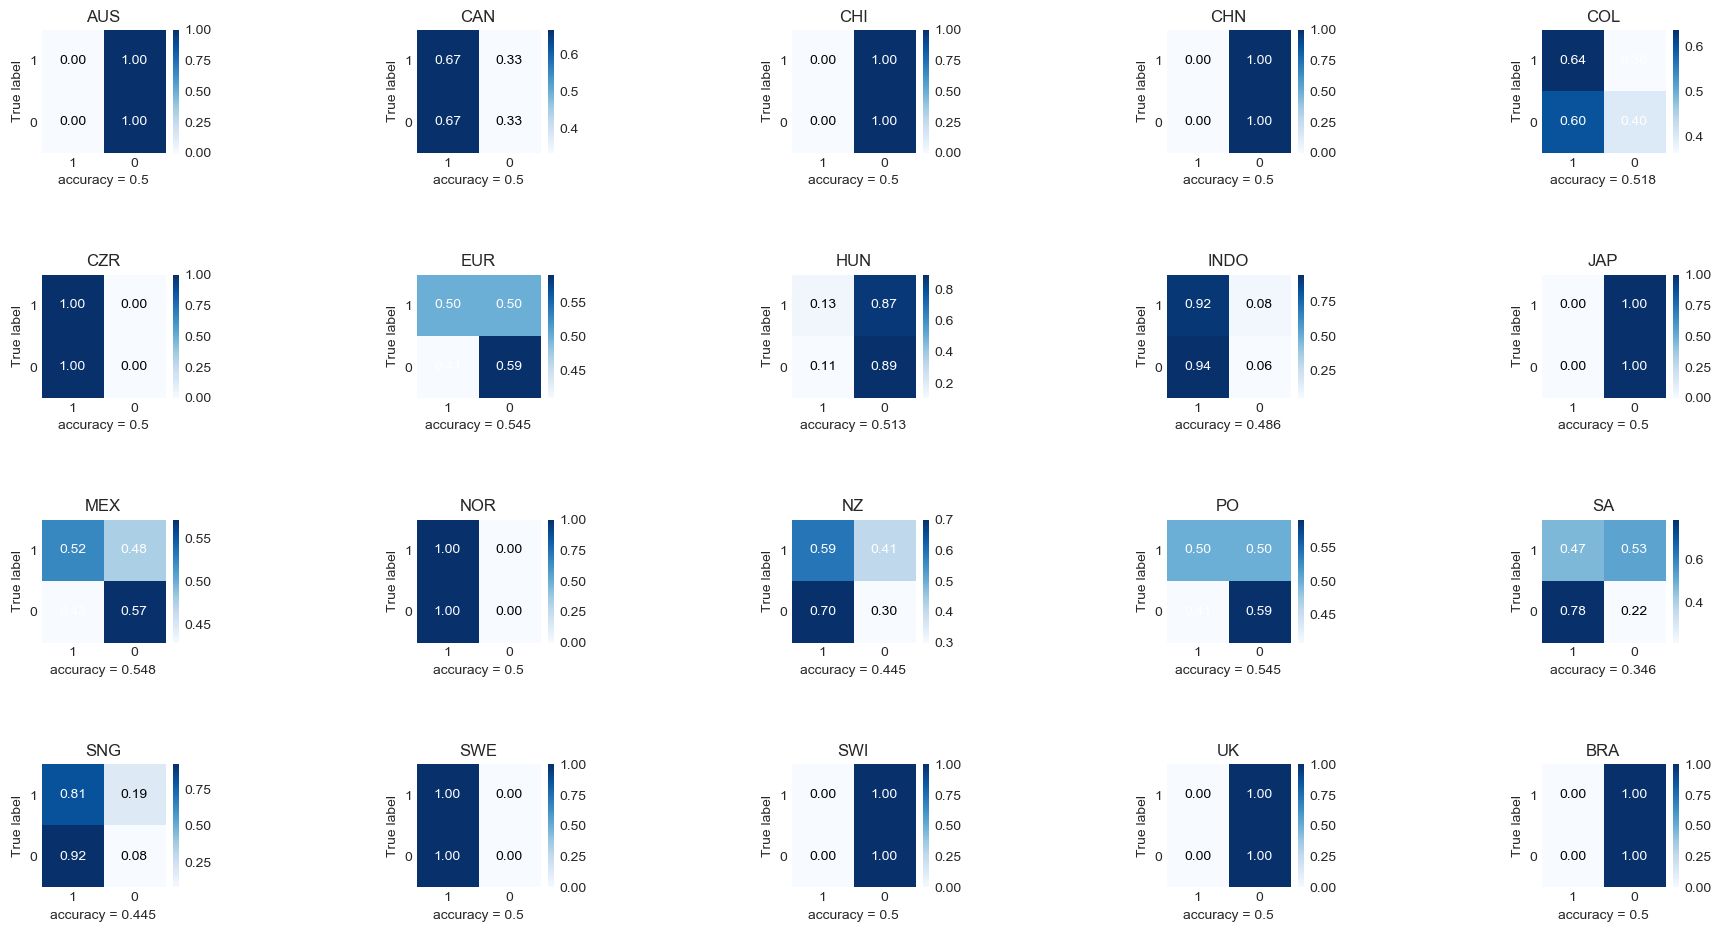
\includegraphics[scale = .30]{images/direction/clf_cm_test.png}
    \caption{SVC Confusion Matrix for all countries for Test Dataset}
    \label{simulationfigure}
\end{figure}

\begin{itemize}
  \item On training dataset most country's models seem to perform better than random walk model (random guess).
  \item On test dataset only a few country's model perform better than random walk, while others being similar to worse than random walk.
  \item It appears that most models created are not generalizable as their in sample performance is way better than their out of sample performance.
  \item It would be interesting to add sentiment and uncertainty variables extracted from FOREX news to the model as they might significantly improve the performance
        of the model as their is a general hypothesis that news articles dictate foreign exchange directional change over the long run.
\end{itemize}


\subsection{Neural Network for Buy/Sell Classification}
\vspace*{5mm}

\subsubsection{Setup}

\vspace*{5mm}

\begin{itemize}
  \item A multi-layer perceptron with 2 hidden layer is created.
  \item The first hidden layer consists of 64 nodes, while the second hidden layer consists of 32 nodes.
  \item RELU activation function is used in the first two layers (best for classification task according to literature) and sigmoid activation function is used in the output
        layer for binary classification.
  \item 1000 epochs were run for each model to repetitively improve the model using back propagation.
  \item Neural Network Models were for all countries, and confusion matrix on the train and test datasets were used to check the performance of our models.
\end{itemize}

\begin{figure}[H]
    \centering
    \hspace*{-1.25in}
    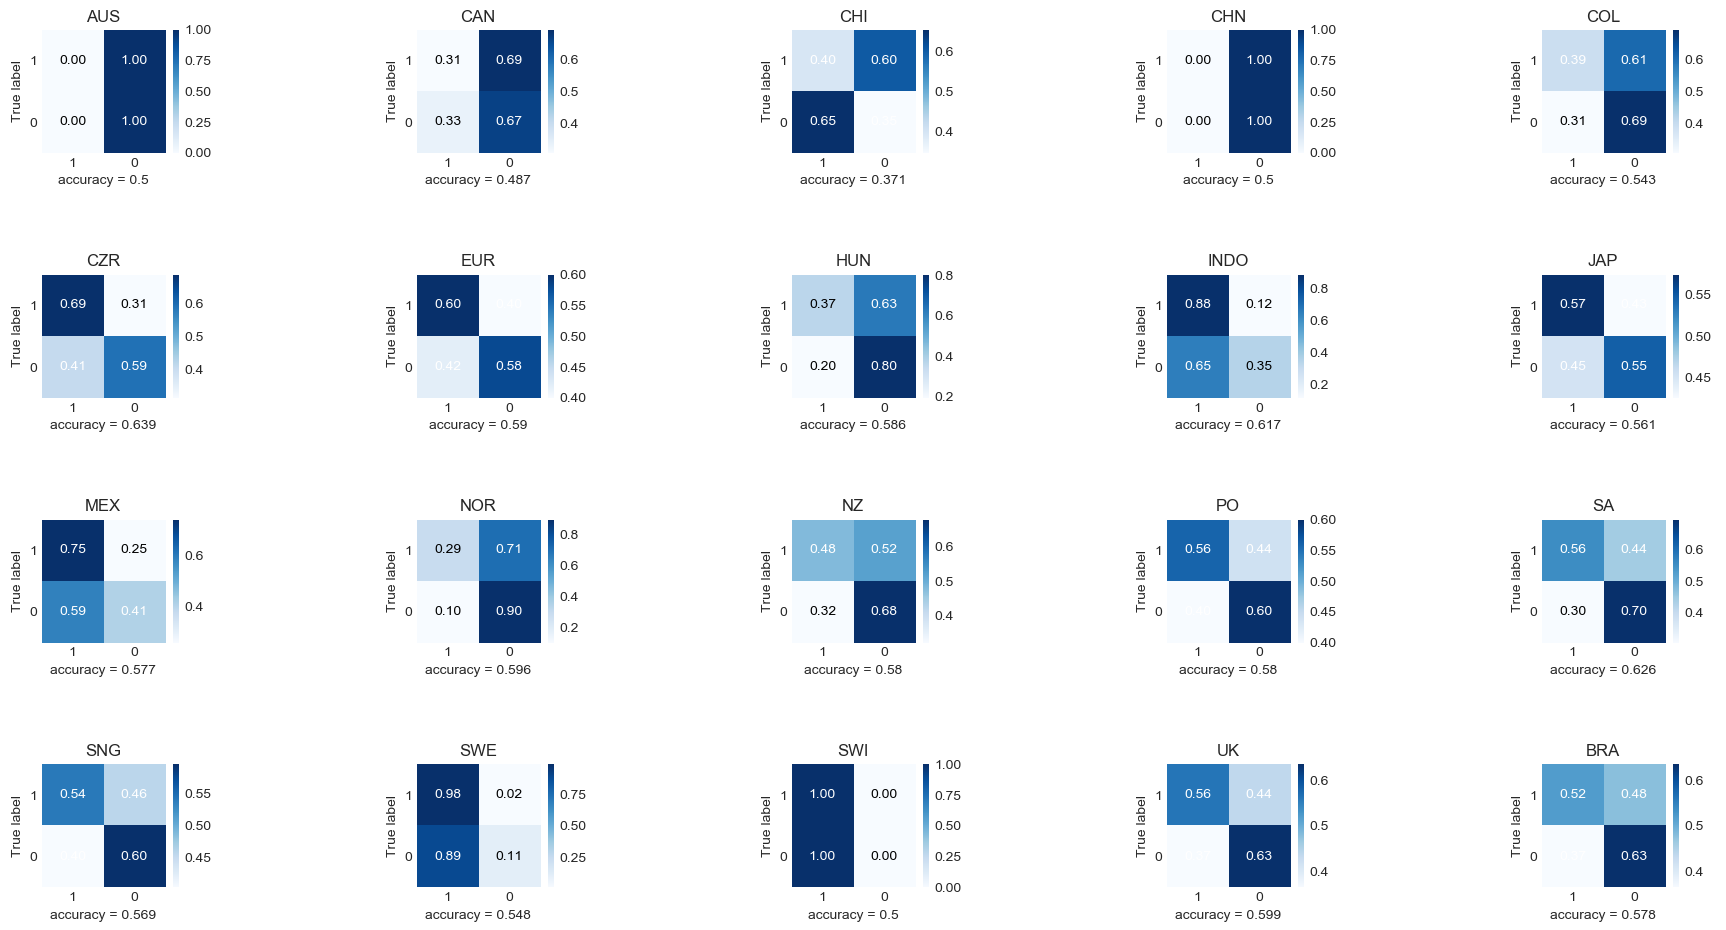
\includegraphics[scale = .30]{images/direction/n_cm_train.png}
    \caption{Neural Network Confusion Matrix for all countries for Training Dataset}
    \label{simulationfigure}
\end{figure}

\begin{figure}[H]
    \centering
    \hspace*{-1.25in}
    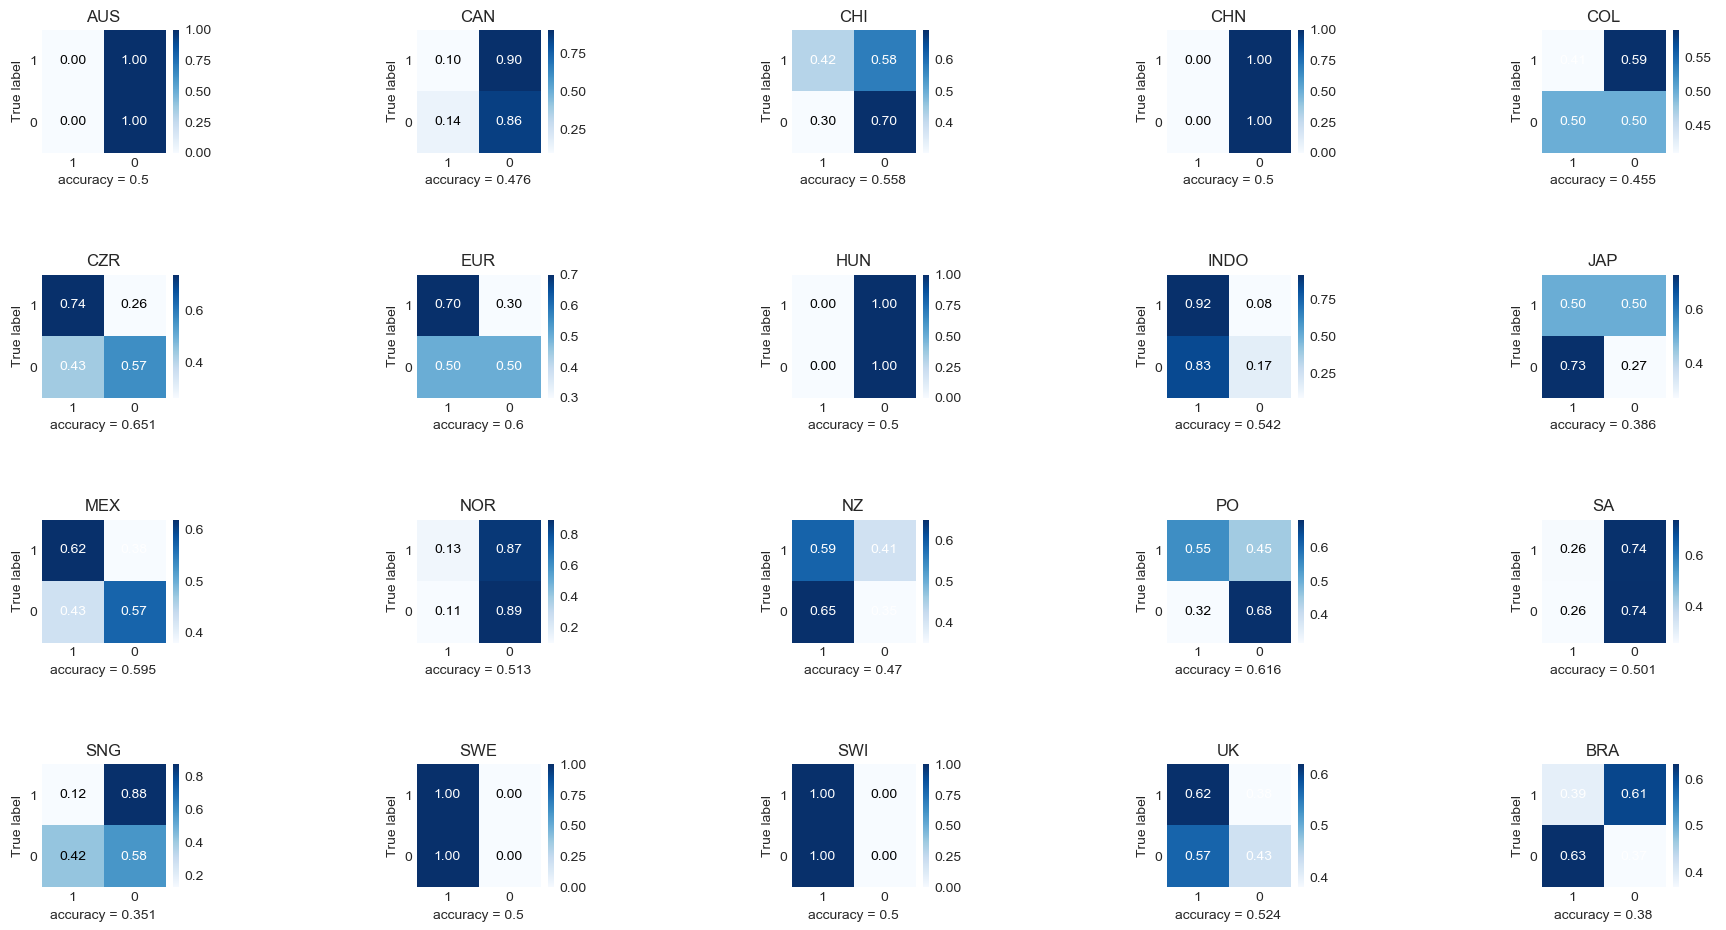
\includegraphics[scale = .30]{images/direction/n_cm_test.png}
    \caption{Neural Network Confusion Matrix for all countries for Test Dataset}
    \label{simulationfigure}
\end{figure}

\begin{itemize}
  \item On training dataset most country's models seem to perform better than random walk model (random guess).
  \item Unlike SVC, on test dataset most countries model still tend to perform better or equal to that of random walk.
  \item It appears that our neural network classifier is more generalizable than our SVC classifier. Although it only manages to beat the random walk in a few cases and be mostly
        equal in others.
  \item It would be interesting to add sentiment and uncertainty variables extracted from FOREX news to the model as they might significantly improve the performance
        of the model as their is a general hypothesis that news articles dictate foreign exchange directional change over the long run. Neural Networks will improve more
        than SVC with sentiment data as deep learning techniques perform better than machine learning technqiues with huge datasets.
\end{itemize}

\end{document}
